\documentclass[aspectratio=169,handout]{beamer}
\usepackage{will_handley_beamer}
\usepackage{title_page}

% Commands
% --------
% - \arxiv{arxiv number}
% - \cols{width}{lh column}{rh column}
% -  \begin{fig(left|right)}[fractional width (e.g 0.6) ]{name of image}
%        content of other column
%    \end{fig(left|right)}

% Talk details
% ------------
\title{Next generation inference tools for cosmology and beyond}
%\subtitle{}
\date{23\textsuperscript{rd} Jan 2024}

\begin{document}

\begin{frame}
    \titlepage
\end{frame}

\begin{frame}
    \frametitle{The golden age of cosmology data}
    \begin{columns}
        \column{0.45\textwidth}
        \begin{itemize}
            \item It's an exciting time to be a cosmologist
            \item Over our research lifetimes we will see next-generation data rates across the electromagnetic spectrum \& beyond:
                \begin{description}
                    \item[Radio] SKA \textit{et al}
                    \item[Micro] SO/CMB-S4
                    \item[IR] JWST, Roman (WFIRST)
                    \item[Optical] Euclid, DESI, Rubin (LSST), EELT
                    \item[X-ray] Athena
                    \item[Gamma-ray] e-ASTROGAM
                    \item[Gravitational] LIGO/Virgo/Kagra + LISA
                    \item[Particle] CTA, IceCube, KM3NeT
                \end{description}
        \end{itemize}
        \column{0.55\textwidth}

        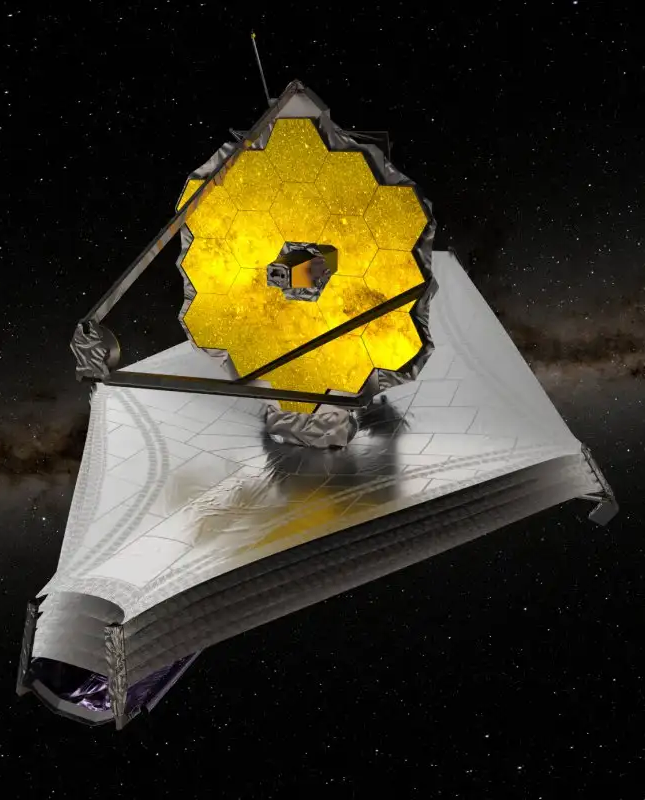
\includegraphics[height=0.15\textwidth]{figures/telescopes/jwst}%
        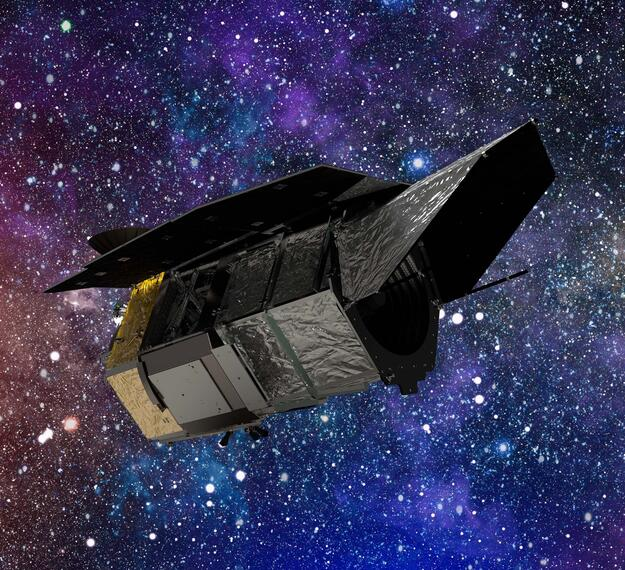
\includegraphics[height=0.15\textwidth]{figures/telescopes/roman}%
        \includegraphics[height=0.15\textwidth]{figures/telescopes/euclid}%
        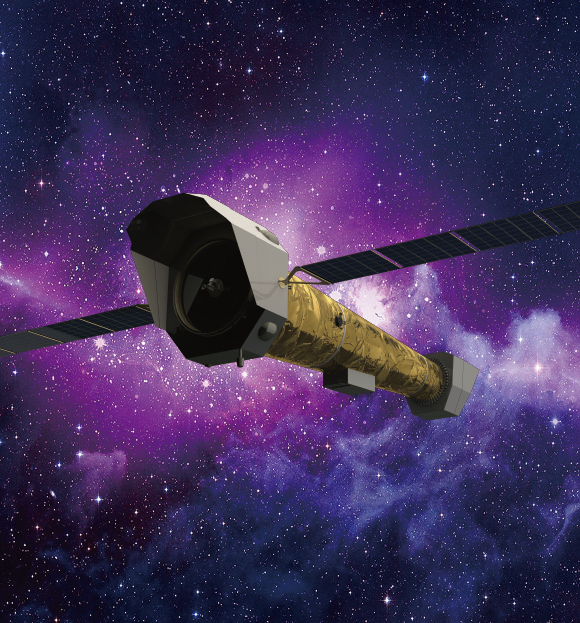
\includegraphics[height=0.15\textwidth]{figures/telescopes/athena}%
        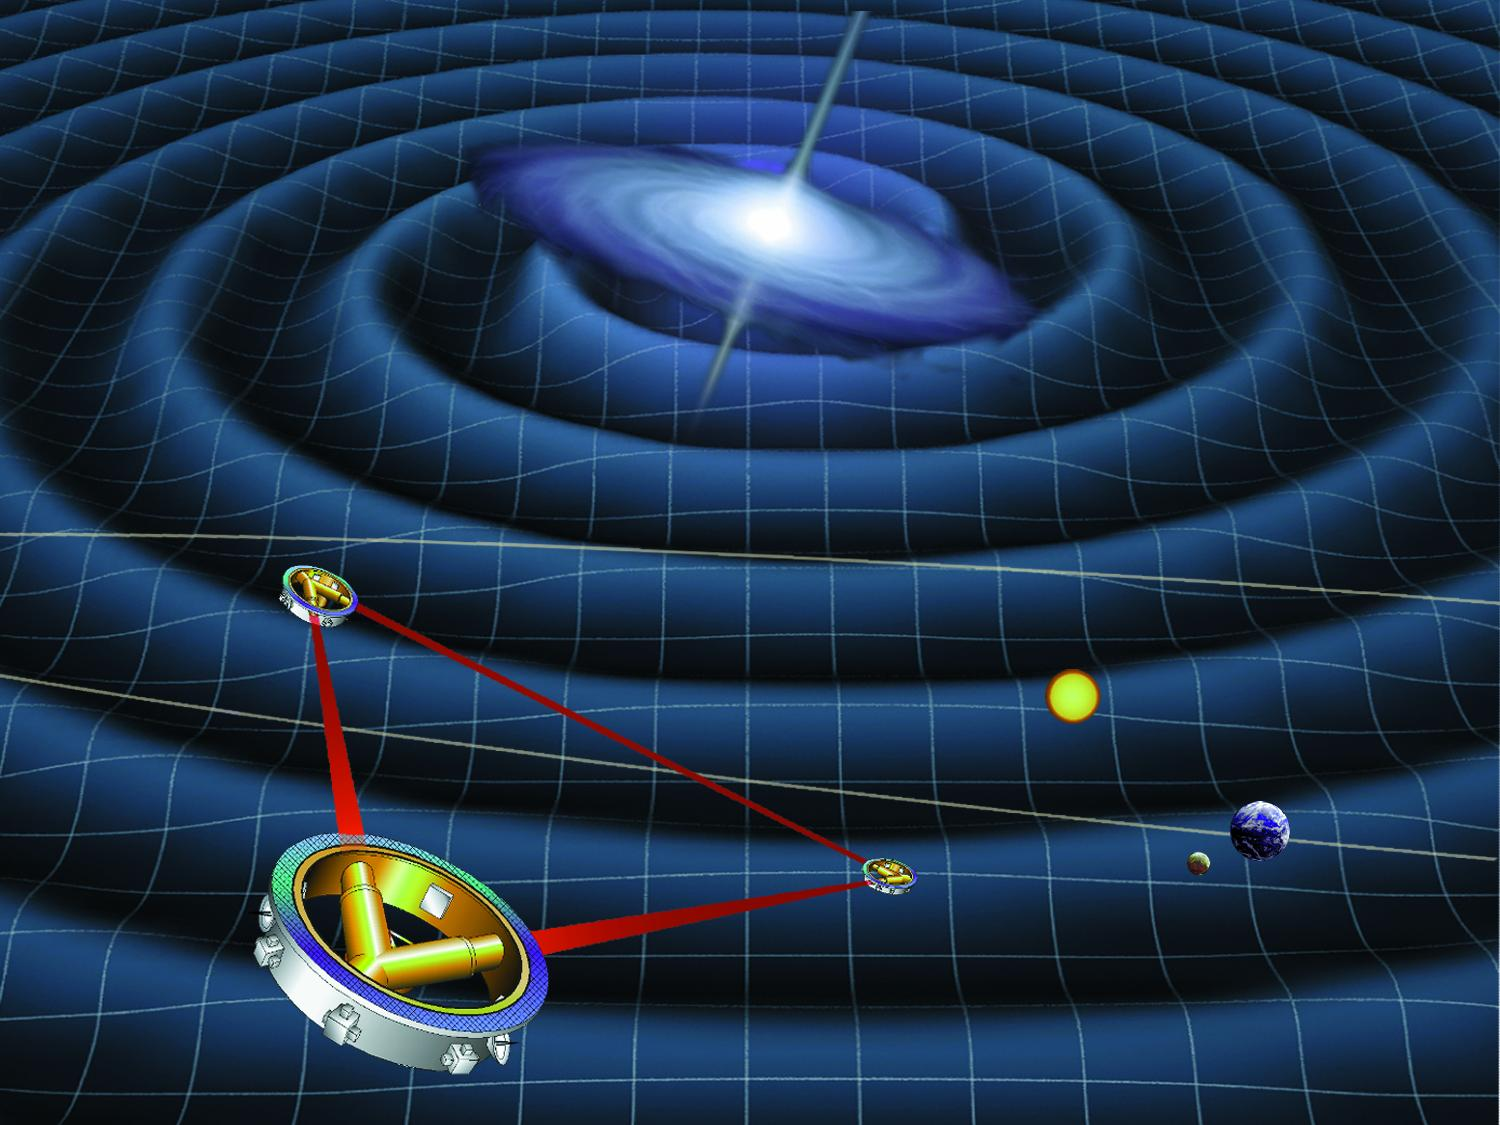
\includegraphics[height=0.15\textwidth]{figures/telescopes/lisa}%
        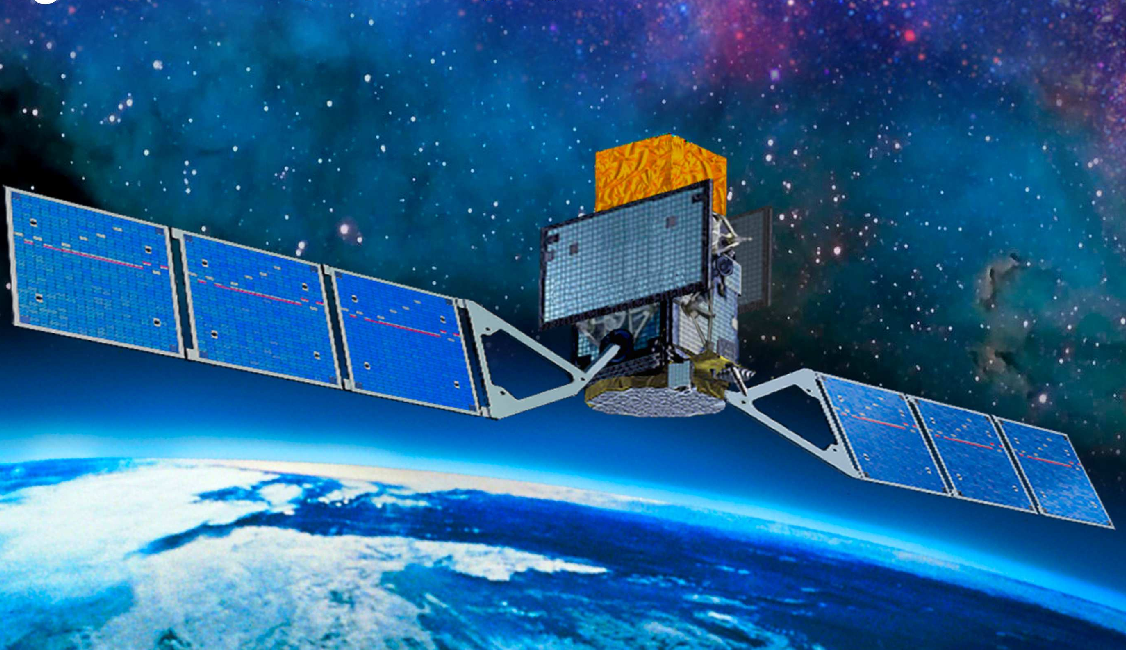
\includegraphics[height=0.15\textwidth]{figures/telescopes/e-ASTROGAM}%

        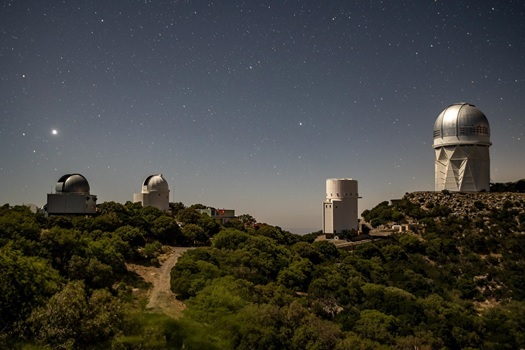
\includegraphics[height=0.16\textwidth]{figures/telescopes/desi}%
        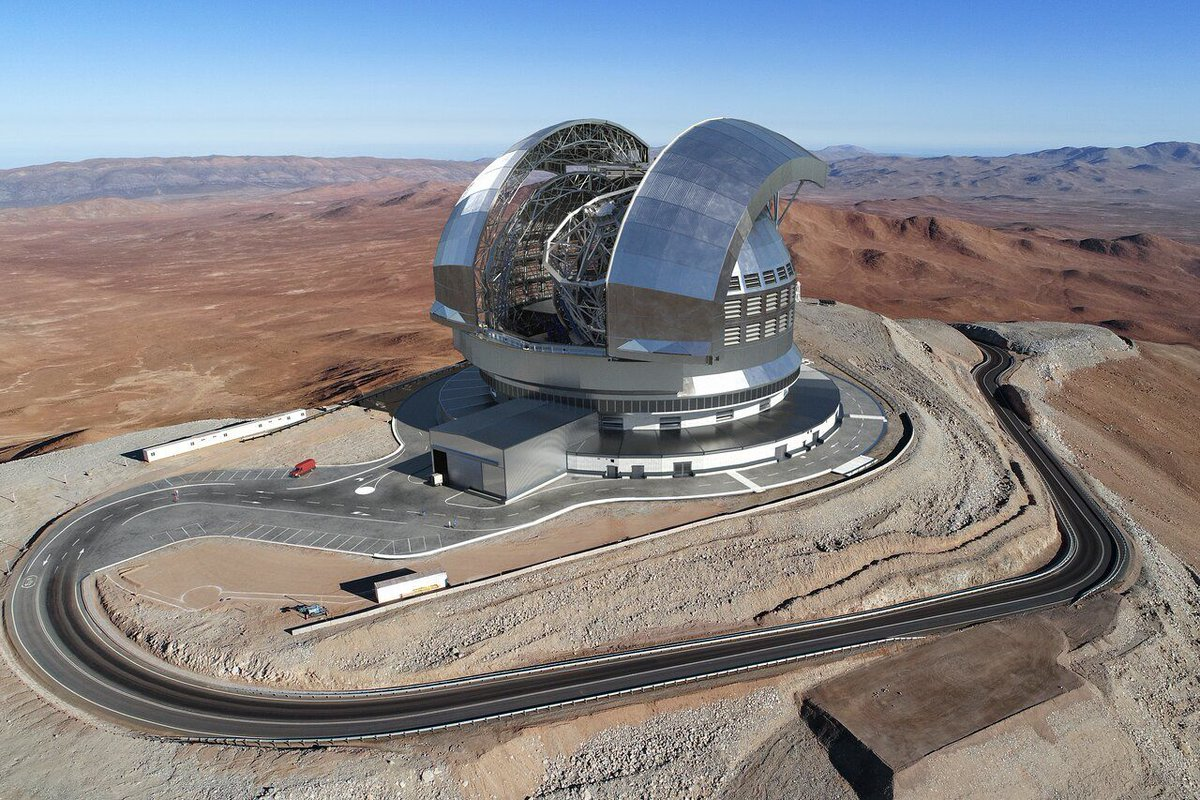
\includegraphics[height=0.16\textwidth]{figures/telescopes/eelt}%
        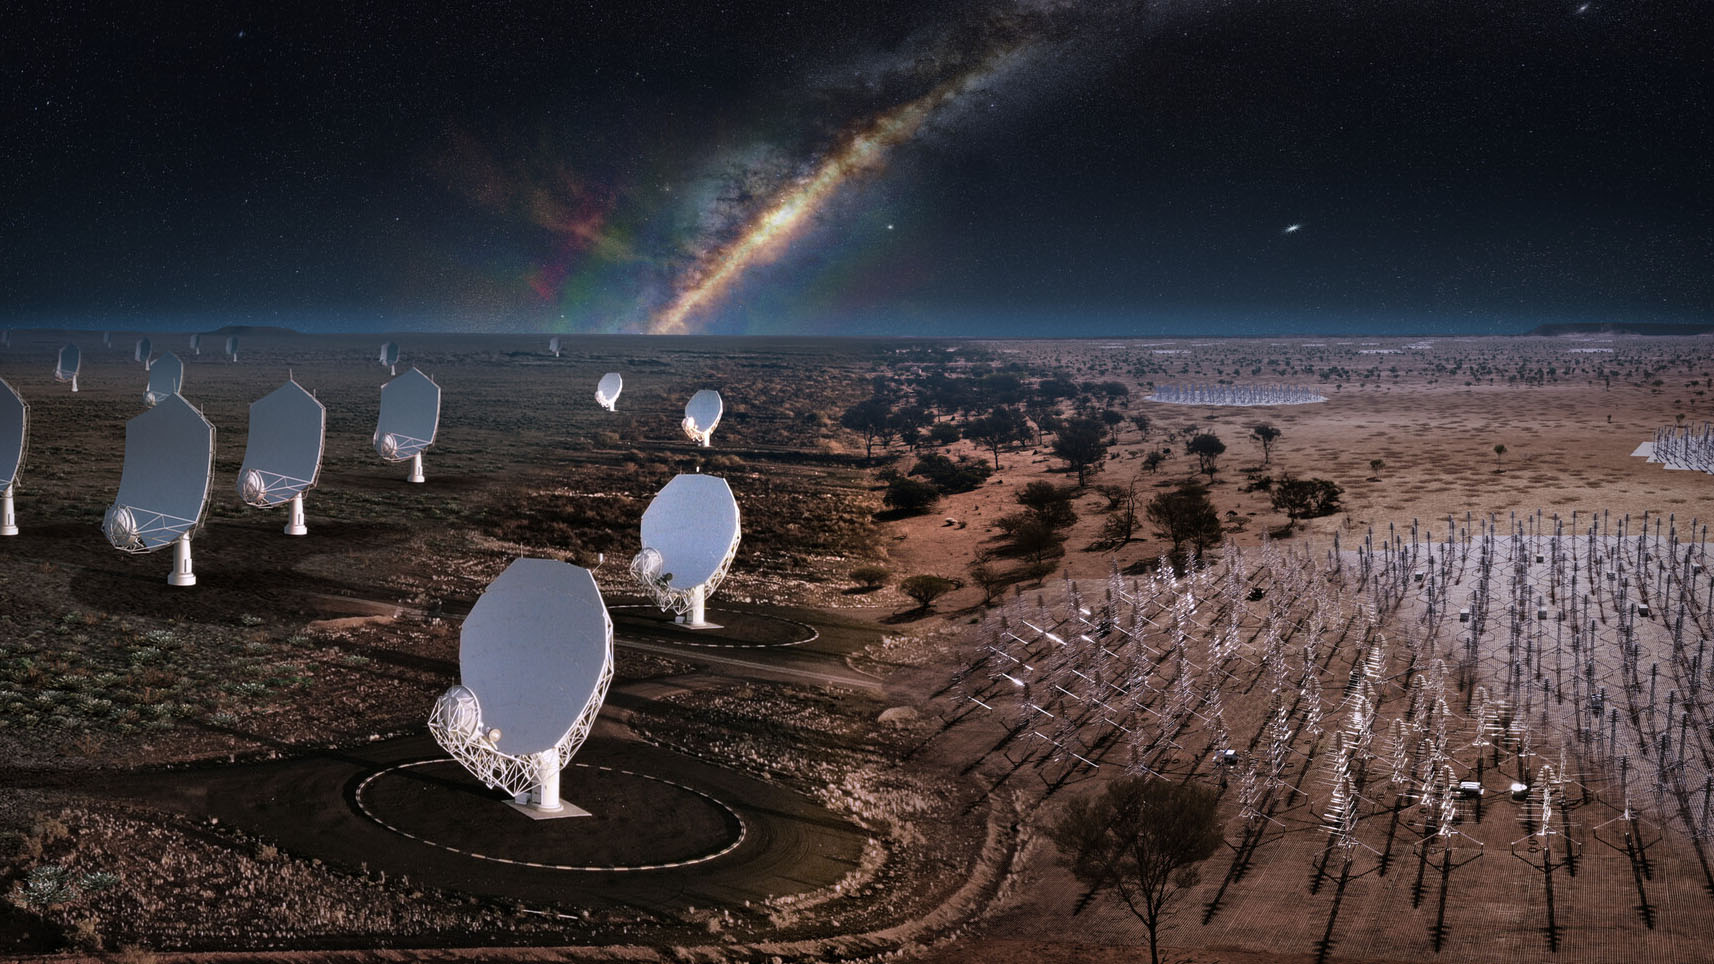
\includegraphics[height=0.16\textwidth]{figures/telescopes/ska}%
        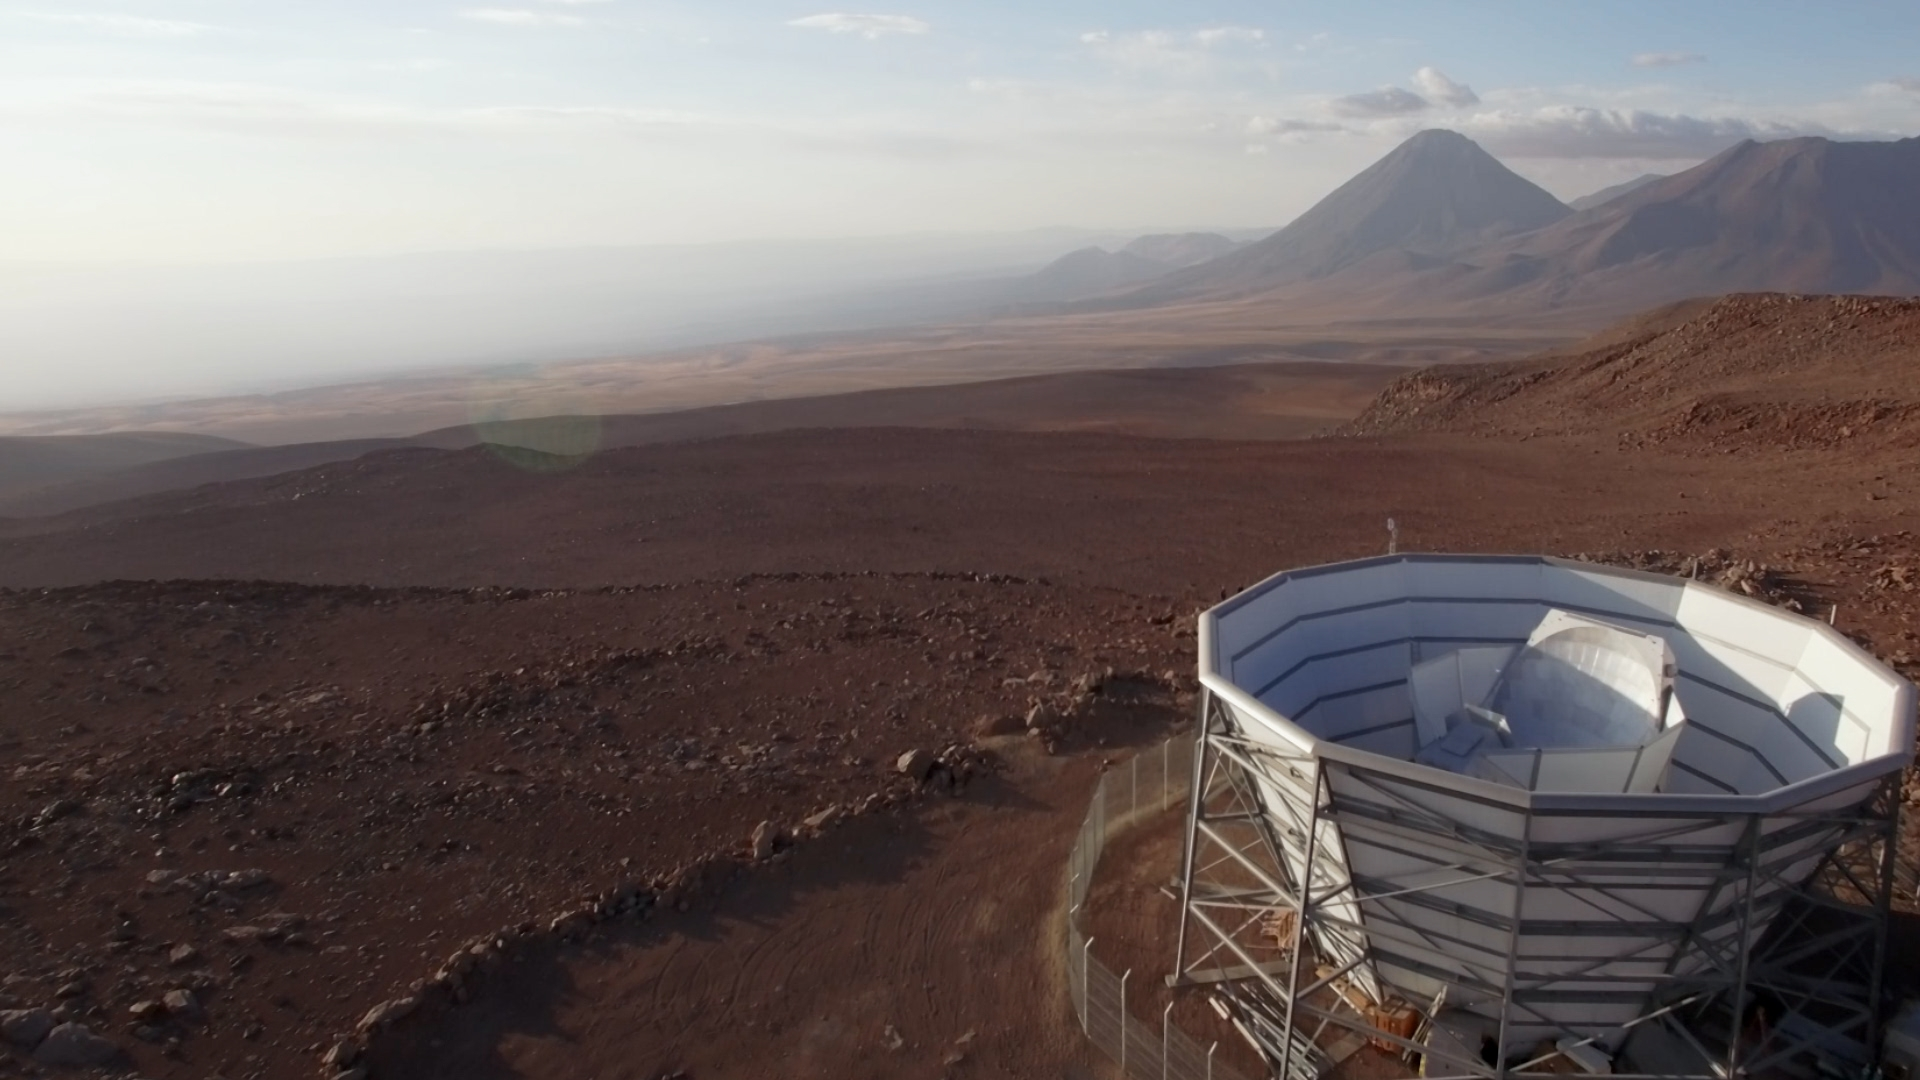
\includegraphics[height=0.16\textwidth]{figures/telescopes/SO}%

        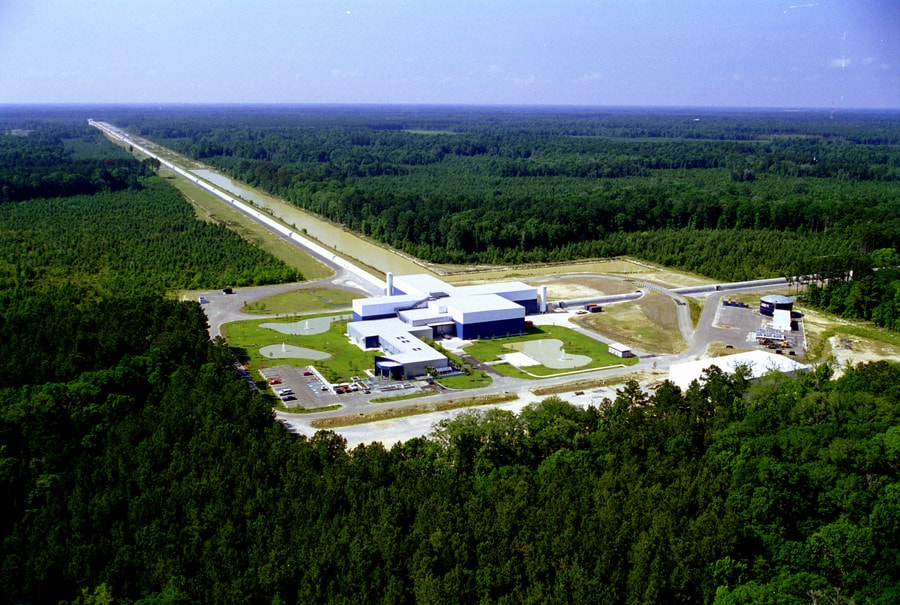
\includegraphics[height=0.191\textwidth]{figures/telescopes/ligo}%
        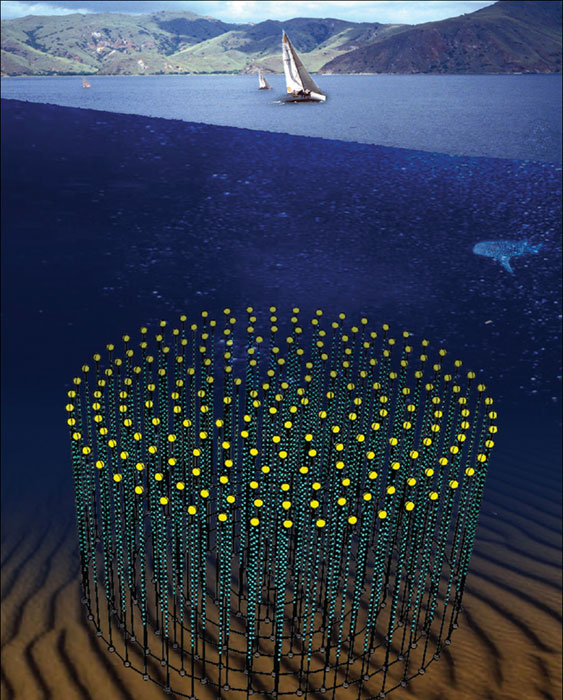
\includegraphics[height=0.191\textwidth]{figures/telescopes/km3n}%
        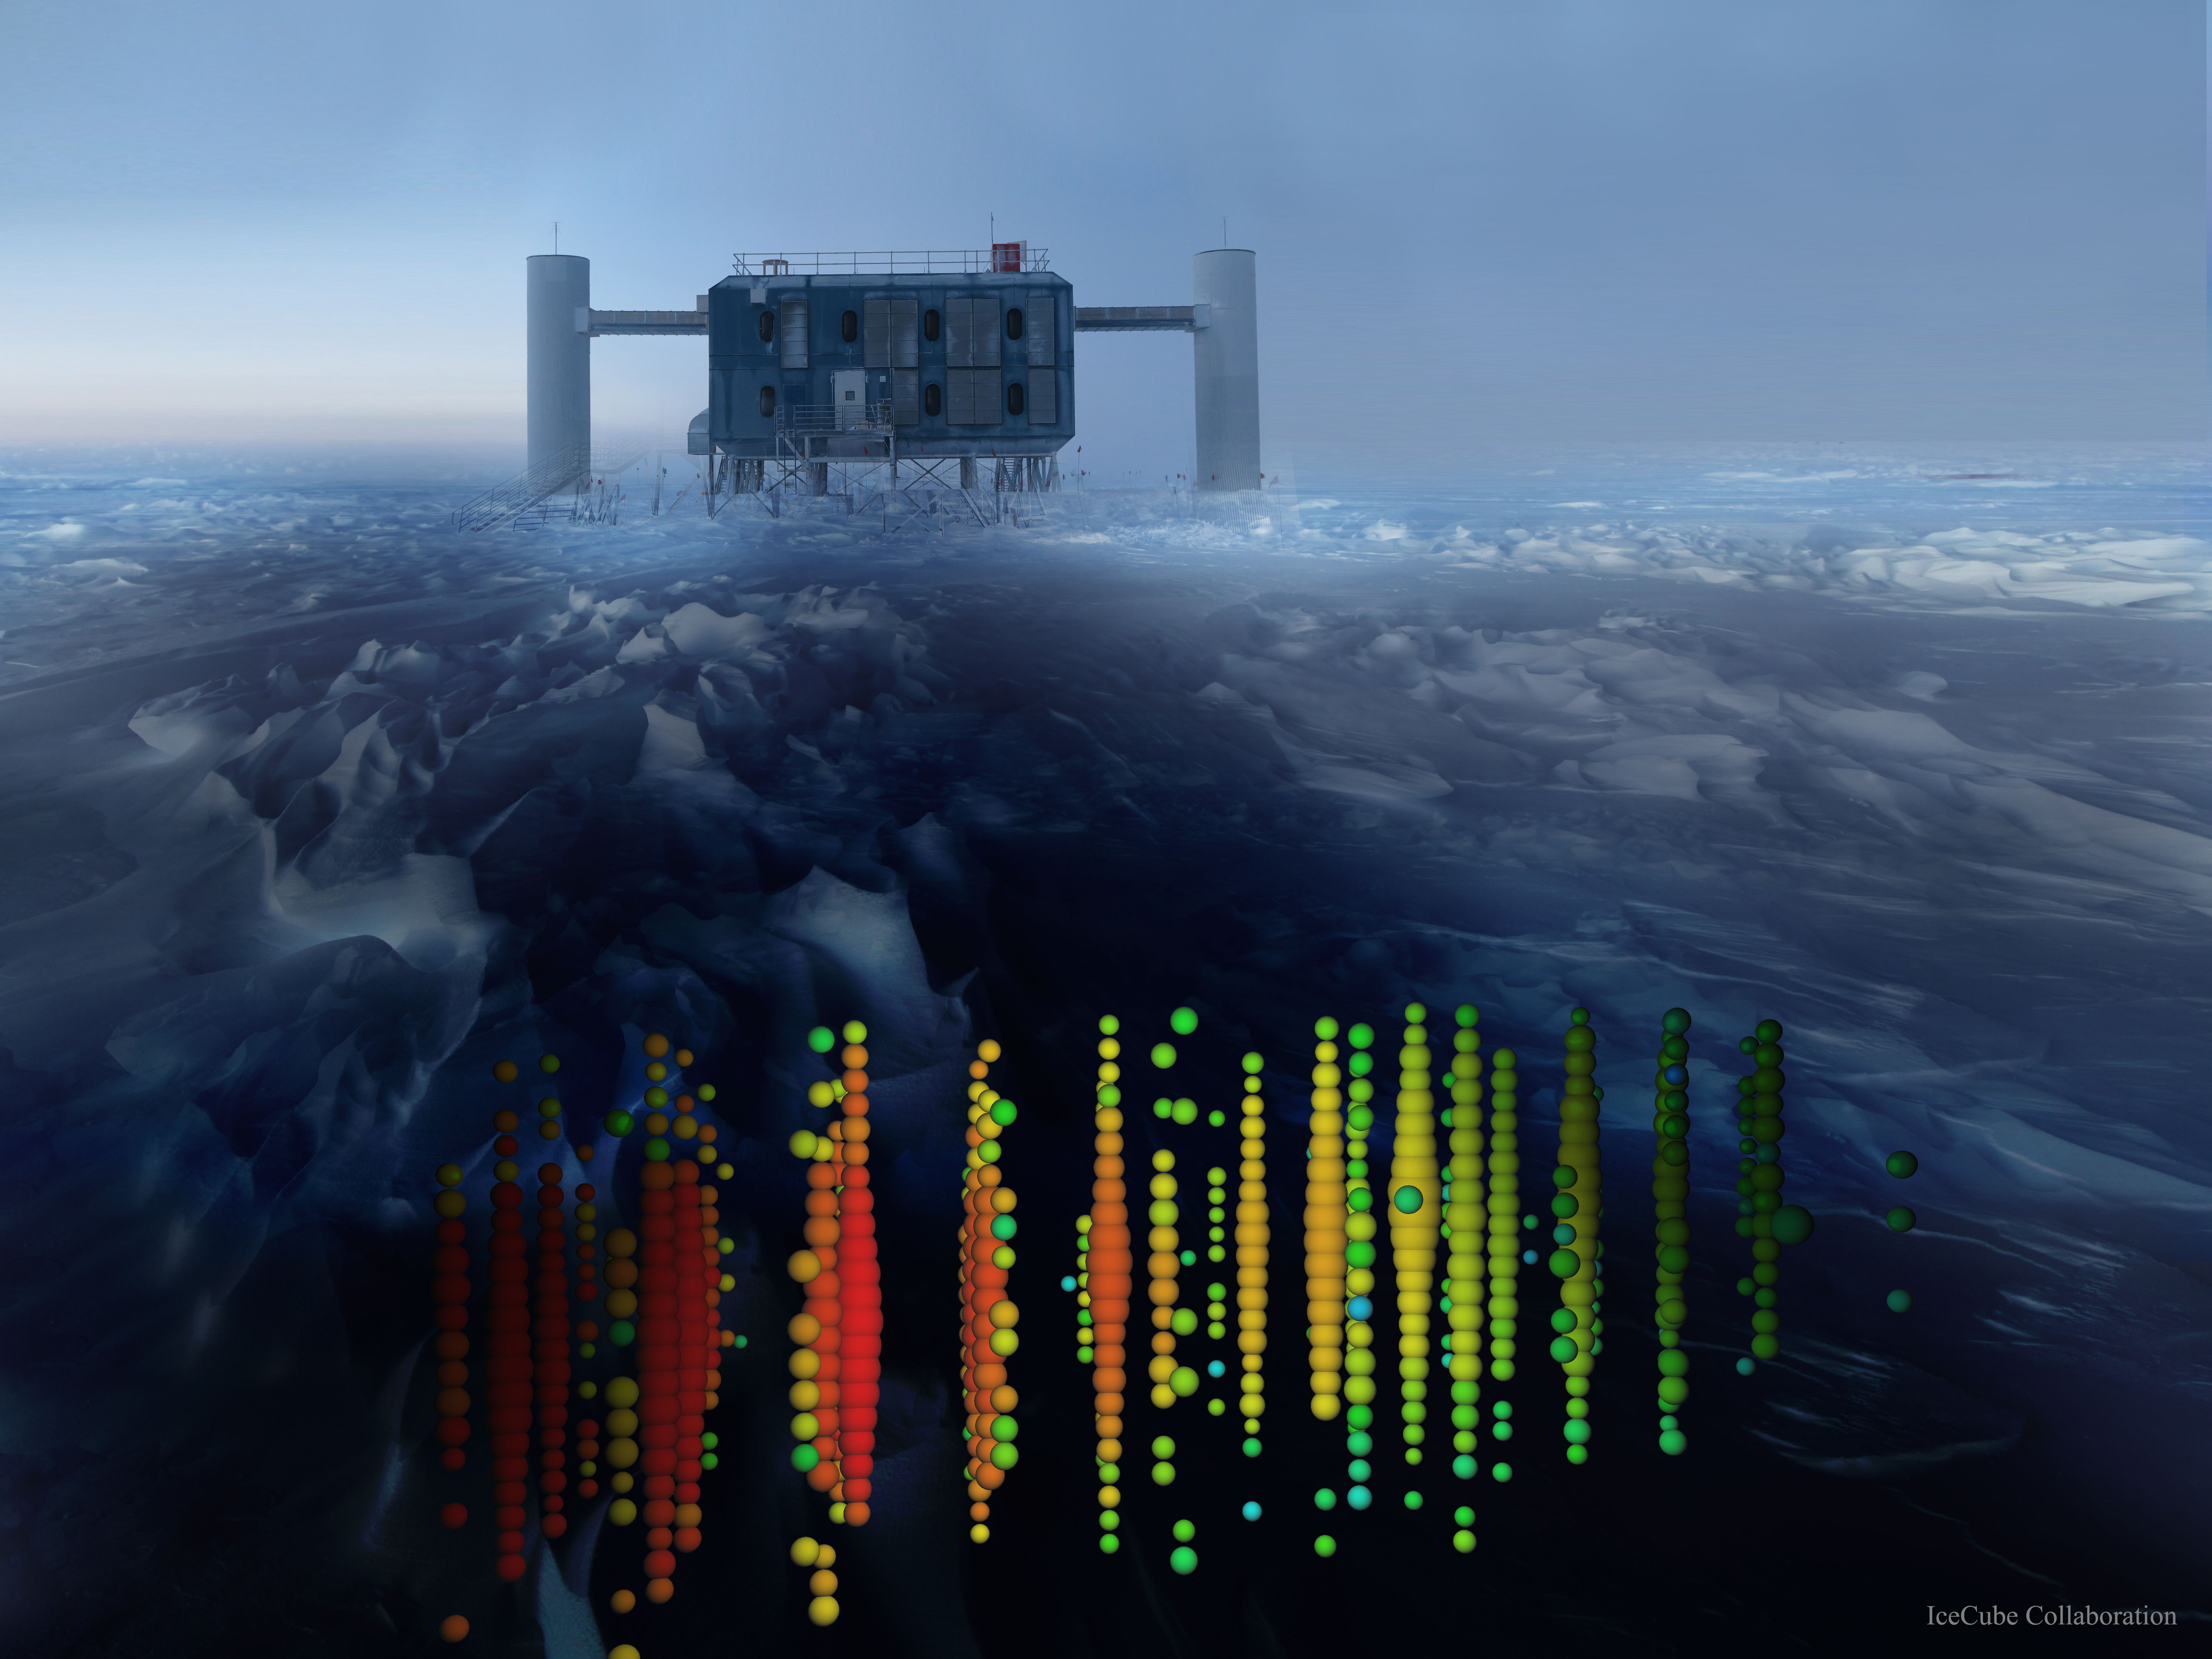
\includegraphics[height=0.191\textwidth]{figures/telescopes/icecube}%
        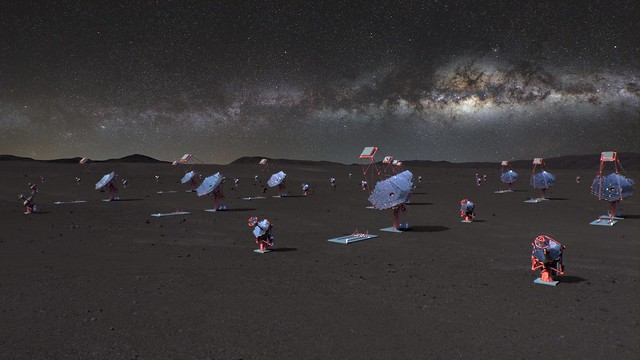
\includegraphics[height=0.191\textwidth]{figures/telescopes/CTA}%

        \begin{itemize}
            \item We are moving from an age of \textbf{precision} cosmology to \textbf{accurate} cosmology.
            \item \textbf{Systematics} $\gtrsim$ \textbf{statistics}.
            \item Software \& tools run the risk of lagging behind hardware
        \end{itemize}
        
    \end{columns}
\end{frame}

\begin{frame}
    \frametitle{Tensions in cosmology}
    \begin{columns}
        \column{0.5\textwidth}
        \begin{itemize}
            \item In addition, a host of ``tensions'' have arisen in cosmology:
            \item \textbf{Data}:
                    $H_0$, $S_8$, $A_L/\Omega_K$, Li
            \item \textbf{Theory}:
                    Initial conditions, Entropy, Dark energy, dark matter, quantum gravity
            \item \textbf{Analysis}:
            \item Disentangling systematics from new physics is challenging!
            \item Almost all cosmological analyses pragmatically assume a fiducial flat $\Lambda$CDM assumption during their analyses.
            \item Unless this is resolved, we risk confirmation bias in the analysis of next-gen data.
        \end{itemize}
        \column{0.5\textwidth}
        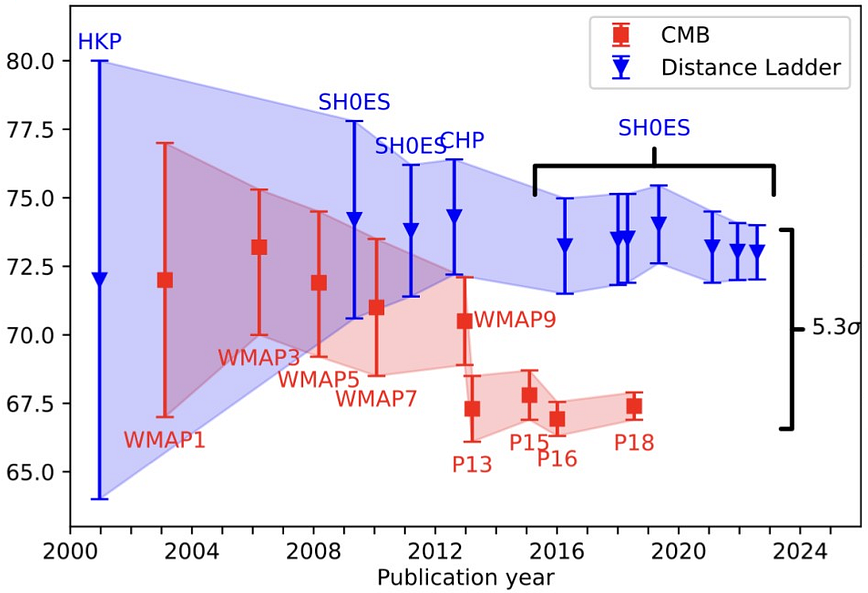
\includegraphics[width=\textwidth]{figures/hubble_tension}
        
    \end{columns}
\end{frame}

\begin{frame}
    \frametitle{Perils ahead}
    \begin{itemize}
        \item Scale of data is daunting (SKA)
        \item Systematics vs statistics
        \item Move from ``precision'' cosmology to ``accurate'' cosmology
        \item Have to assume a model
    \end{itemize}
\end{frame}

\begin{frame}
    \frametitle{<+Bayesian slide+>}
    \begin{itemize}
        \item Bayes theorem
    \end{itemize}
        \[
                P(\theta|D) = \frac{P(D|\theta)P(\theta)}{P(D)}
        \]
        \[
            \qquad
            \text{Posterior} = \frac{\text{Likelihood}\times\text{Prior}}{\text{Evidence}}
        \]
        \[
                \mathcal{P}(\theta|D) = \frac{\mathcal{L}(D|\theta)\pi(\theta)}{\mathcal{Z}(D)}
            \qquad
            \text{Posterior} = \frac{\text{Likelihood}\times\text{Prior}}{\text{Evidence}}
        \]
        \[
                \mathcal{P}\times\mathcal{Z} = \mathcal{L}\times\pi
            \]
            \[
                \mathcal{P}\times\mathcal{Z} = \mathcal{J} = \mathcal{L}\times\pi, \qquad \text{Joint} = \mathcal{J} = P(D,\theta)
            \]
            \[r = \frac{\mathcal{J}}{\pi\times\mathcal{Z}} = \frac{\mathcal{L}}{\mathcal{Z}} = \frac{\mathcal{P}}{\pi}\]
\end{frame}

\begin{frame}
    \frametitle{Applications: The three pillars of Bayesian inference}
    \begin{columns}[t]
        \column{0.33\textwidth}
        \begin{block}{Parameter estimation}
            What do the data tell us about the parameters of a model?

            \textit{e.g. the size or age of a $\Lambda$CDM universe}
            \[ \hspace{-4pt}\C[0]{P(\theta|D,M)} = \frac{\C[2]{P(D|\theta,M)} \C[1]{P(\theta|M)}}{\C[3]{P(D|M)}} \] 
            \[ \C[0]{\mathcal{P}} = \frac{\C[2]{\mathcal{L}} \times\C[1]{\pi}}{\C[3]{\mathcal{Z}}}\] 
            \[ \C[0]{\text{Posterior}} = \frac{\C[2]{\text{Likelihood}} \times\C[1]{\text{Prior}}}{\C[3]{\text{Evidence}}}\]
        \end{block}
        \column{0.3\textwidth}
        \begin{block}{Model comparison}
            How much does the data support a particular model?

            \textit{e.g. $\Lambda$CDM vs a dynamic dark energy cosmology}
            \[ \C[4]{P(M|D)} = \frac{\C[3]{P(D|M)} \C[5]{P(M)}}{\C[7]{P(D)}} \vspace{-7pt}\]
            \[ \frac{\C[3]{\mathcal{Z}_\mathcal{M}} \C[5]{\Pi_\mathcal{M}}}{\C[7]{\sum_m Z_m \Pi_m}} \]
            \[ \C[4]{\text{Posterior}} = \frac{\C[3]{\text{Evidence}} \times\C[5]{\text{Prior}}}{\C[7]{\text{Normalisation}}}\]
        \end{block}
        \column{0.33\textwidth}
        \begin{block}{Tension quantification}
            Do different datasets make consistent predictions from the same model? 
            \textit{e.g. CMB vs Type IA supernovae data}
            \[ \mathcal{R} = \frac{\C[3]{\mathcal{Z}}_{AB}}{\C[3]{\mathcal{Z}}_A\C[3]{\mathcal{Z}}_\mathcal{B}}\] 
            \[
                \begin{aligned} \log\mathcal{S} = \av[{\C[0]{\mathcal{P}}_{AB}}]{\C[2]{\log\mathcal{L}}_{AB}}&\\
                    -\av[{\C[0]{\mathcal{P}}_{A}}]{\C[2]{\log\mathcal{L}}_{A}}&\\
                    -\av[{\C[0]{\mathcal{P}}_{B}}]{\C[2]{\log\mathcal{L}}_{B}}&
                \end{aligned}
            \]
        \end{block}
    \end{columns}
\end{frame}

\begin{frame}
    \frametitle{LBI: Likelihood-based inference}
    \begin{columns}
        \column{0.5\textwidth}
The standard approach if you are fortunate enough to have a likelihood function $\mathcal{L}(\theta|D)$: 
        \begin{enumerate}
            \item Define prior $\pi(\theta)$ 
                \begin{itemize}
                    \item spend some time being philosophical
                \end{itemize}
            \item Sample posterior $\mathcal{P}(\theta|D)$ 
                \begin{itemize}
                    \item use out-of-the-box MCMC tools such as\\ \texttt{emcee} or \texttt{MultiNest}
                    \item make some triangle plots
                \end{itemize}
            \item Optionally compute evidence $\mathcal{Z}(D)$
                \begin{itemize}
                    \item e.g. nested sampling or parallel tempering
                    \item do some model comparison (i.e. science)
                    \item talk about tensions e.g. \arxiv{2401.02929}
                \end{itemize}
        \end{enumerate}
        \column{0.5\textwidth}
        \hfill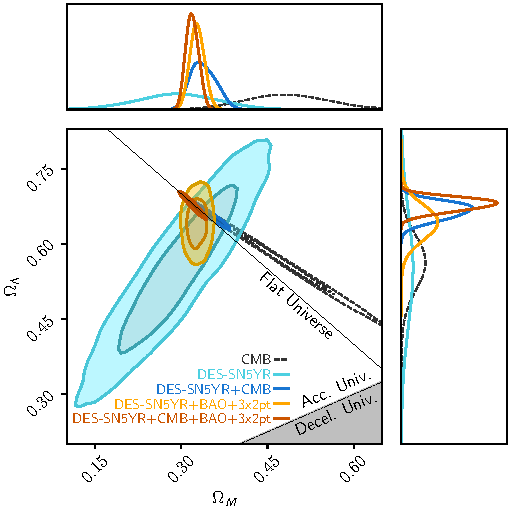
\includegraphics[width=0.6\textwidth]{figures/des_parameters.pdf}
        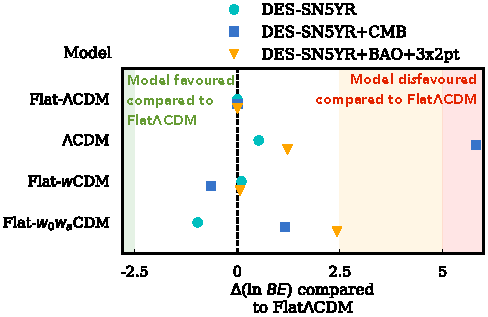
\includegraphics[width=0.5\textwidth]{figures/des_model_comparison.pdf}%
        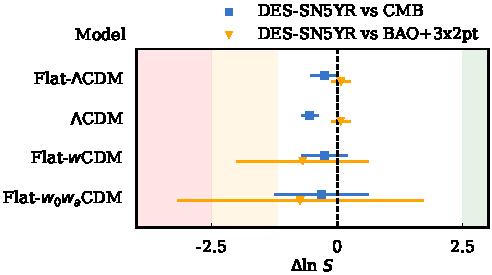
\includegraphics[width=0.5\textwidth]{figures/des_suspiciousness.pdf}
    \end{columns}
\end{frame}

\begin{frame}
    \frametitle{SBI: Simulation-based inference}
    \begin{columns}
        \column{0.5\textwidth}
        \begin{itemize}
            \item Only have access to a forward model $\theta \rightarrow D$.
            \item $(\theta,D)$ plane gives a more expansive theoretical view of inference.
            \item Forward model defines \emph{implicit} likelihood~$\mathcal{L}$:
            \item Simulator generates samples from $\mathcal{L}(D|\theta)$.
            \item With a prior $\pi(\theta)$ can generate samples from joint distribution~$\mathcal{J}(\theta,D)=\mathcal{L}(D|\theta)\pi(\theta)$\\\hfill \emph{the ``probability of everything''}.
            \item Task of SBI is then to go from joint~$\mathcal{J}$ to posterior $\mathcal{P}(\theta|D)$ and evidence $\mathcal{Z}(D)$ -- and possibly likelihood $\mathcal{L}(D|\theta)$.
            \item SBI \& forward modelling force us to think about data space~$D$ \& parameter space~$\theta$.
        \end{itemize}
        \column{0.5\textwidth}
        \includegraphics<1>[page=1, width=\textwidth]{figures/sbi_parameter_estimation.pdf}%
        \includegraphics<2>[page=2, width=\textwidth]{figures/sbi_parameter_estimation.pdf}%
        \includegraphics<3>[page=3, width=\textwidth]{figures/sbi_parameter_estimation.pdf}%
        \includegraphics<4>[page=4, width=\textwidth]{figures/sbi_parameter_estimation.pdf}%
        \includegraphics<5>[page=5, width=\textwidth]{figures/sbi_parameter_estimation.pdf}%
    \end{columns}
\end{frame}


\begin{frame}
    \frametitle{Simulation-based inference \& model comparison}
    \begin{columns}
        \column{0.3\textwidth}
        \begin{itemize}
            \item Extend: models $A$ and $B$.
            \item Each with own separate parameters $\theta_A$ and $\theta_B$ (can be same).
            \item The evidence $\mathcal{Z}(D|M)$ compares models
            \item Occams razor: more~predictive $\equiv$~more~probable \\(due to normalisation).
        \end{itemize}
        
        \column{0.7\textwidth}
        \includegraphics<1>[page=1, width=\textwidth]{figures/sbi_model_comparison.pdf}%
        \includegraphics<2>[page=2, width=\textwidth]{figures/sbi_model_comparison.pdf}%
        \includegraphics<3>[page=3, width=\textwidth]{figures/sbi_model_comparison.pdf}%
    \end{columns}
\end{frame}


\begin{frame}
    \frametitle{Conclusions}
    \framesubtitle{\href{https://www.github.com/handley-lab}{github.com/handley-lab}}
    \tikz[overlay,remember picture]
        \node[anchor=north east] (A) at ($(current page.north east)+(0,0)$) {
            
\includegraphics[width=0.09\textheight]{figures/students/adam_ormondroyd.jpg}%
            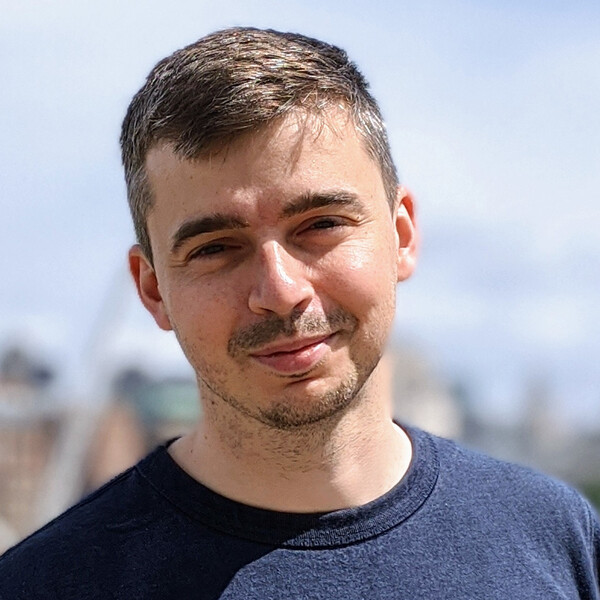
\includegraphics[width=0.09\textheight]{figures/students/david_yallup.jpg}%
            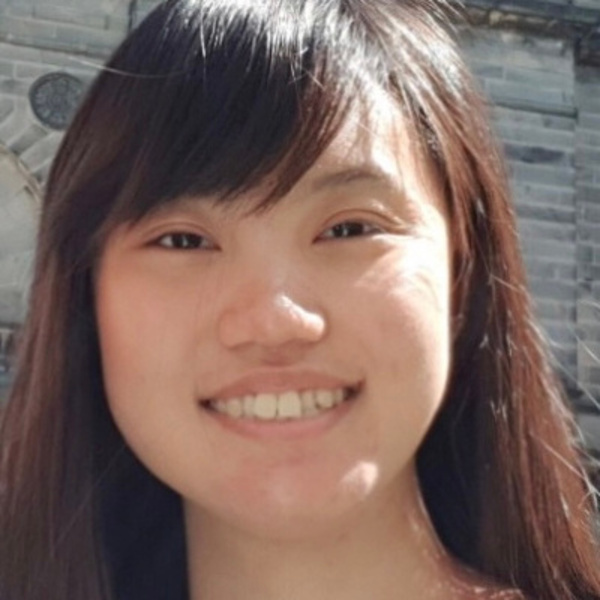
\includegraphics[width=0.09\textheight]{figures/students/dily_ong.jpg}%
            
\includegraphics[width=0.09\textheight]{figures/students/felicity_ibrahim.jpg}%
            
\includegraphics[width=0.09\textheight]{figures/students/george_carter.jpg}%
            
\includegraphics[width=0.09\textheight]{figures/students/harry_bevins.jpg}%
            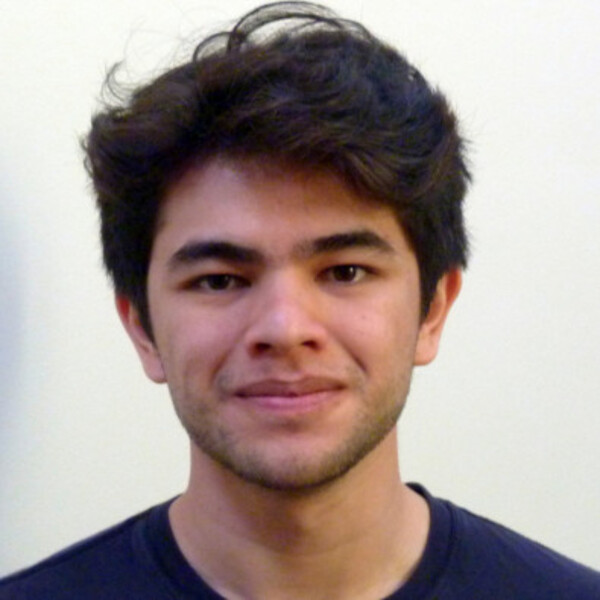
\includegraphics[width=0.09\textheight]{figures/students/ian_roque.jpg}%
            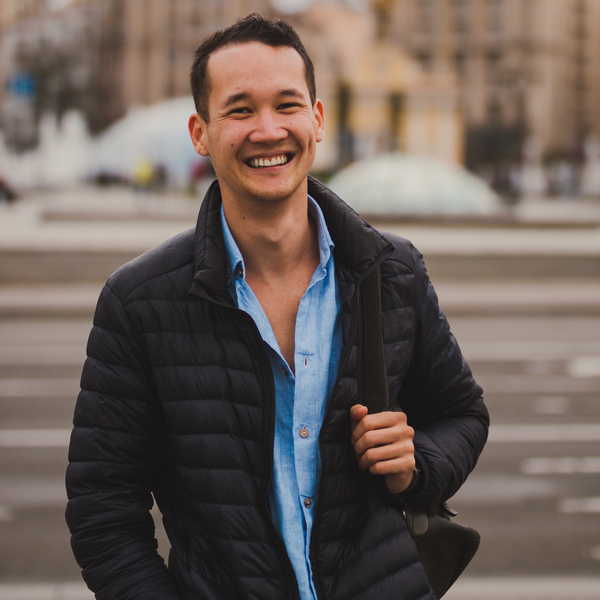
\includegraphics[width=0.09\textheight]{figures/students/kilian_scheutwinkel.jpg}%
            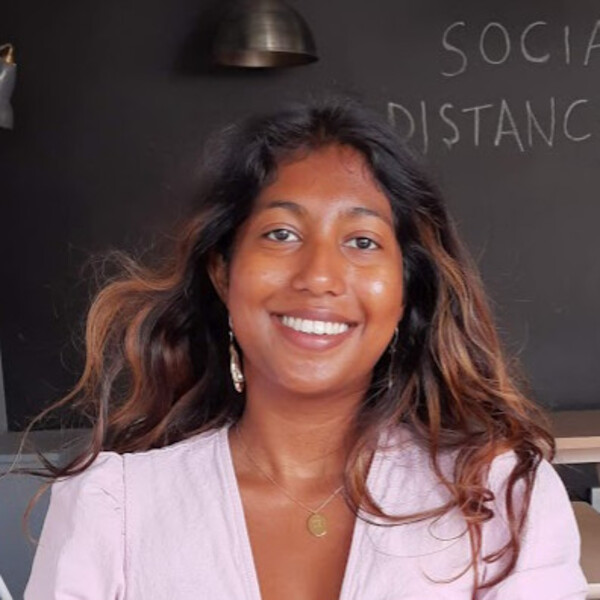
\includegraphics[width=0.09\textheight]{figures/students/metha_prathaban.jpg}%
            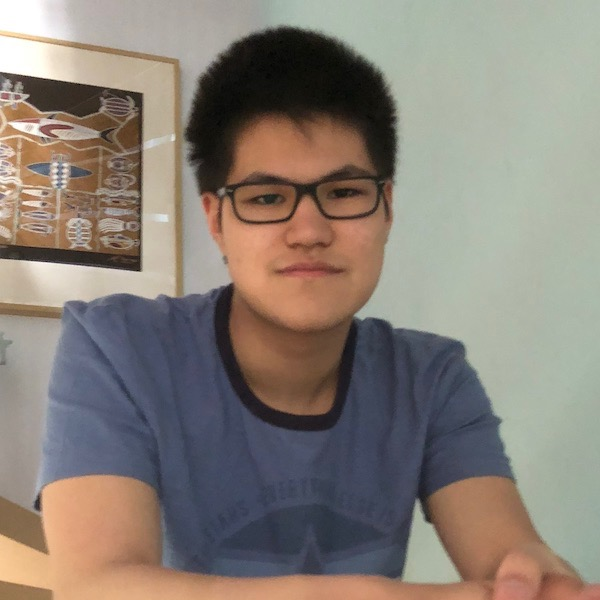
\includegraphics[width=0.09\textheight]{figures/students/namu_kroupa.jpg}%
            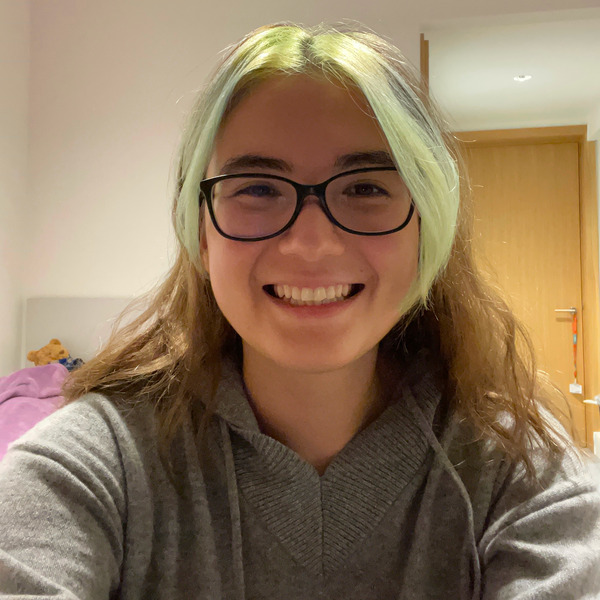
\includegraphics[width=0.09\textheight]{figures/students/sinah_legner.jpg}%
            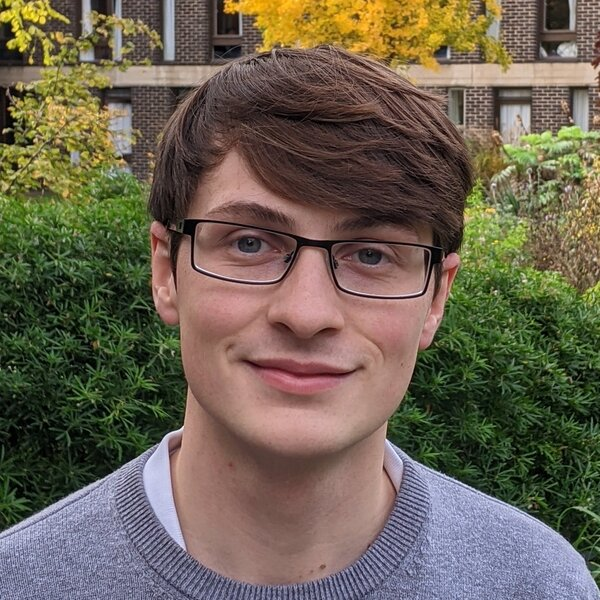
\includegraphics[width=0.09\textheight]{figures/students/thomas_gessey-jones.jpg}%
            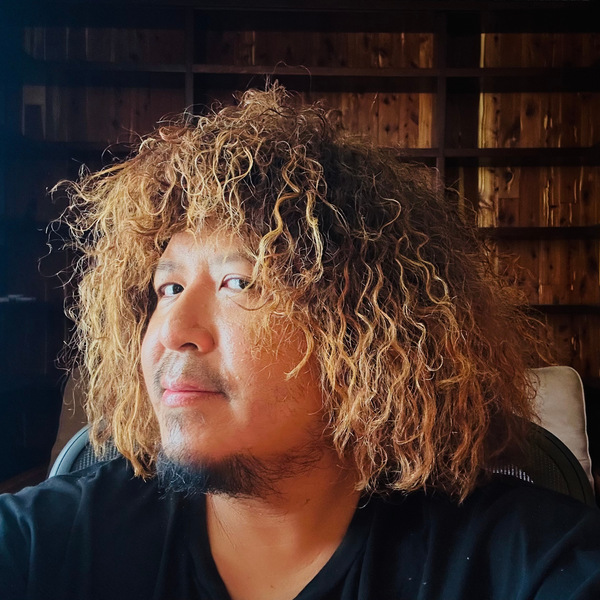
\includegraphics[width=0.09\textheight]{figures/students/tze_goh.jpg}%
            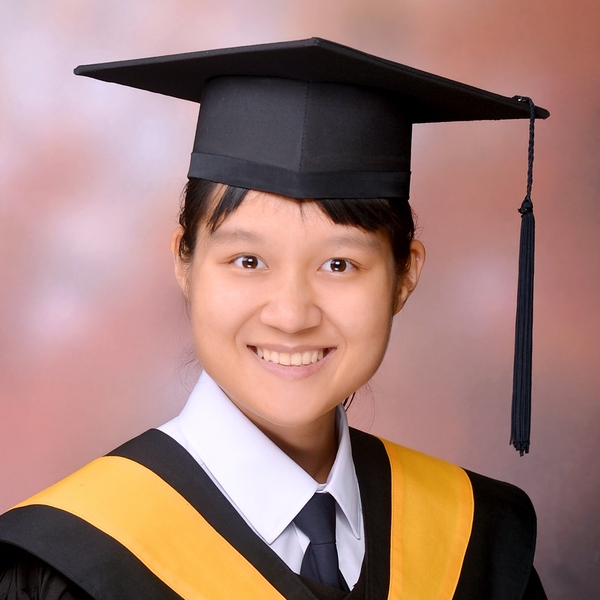
\includegraphics[width=0.09\textheight]{figures/students/wei-ning_deng.jpg}%
    };
\end{frame}

\end{document}
